\documentclass[spanish]{textolivre}

% metadata
\journalname{Texto Livre}
\thevolume{17}
%\thenumber{1} % old template
\theyear{2024}
\receiveddate{\DTMdisplaydate{2024}{2}{27}{-1}}
\accepteddate{\DTMdisplaydate{2024}{4}{17}{-1}}
\publisheddate{\today}
\corrauthor{Manuel Fernando Ramos Nunez}
\articledoi{10.1590/1983-3652.2024.51392}
%\articleid{NNNN} % if the article ID is not the last 5 numbers of its DOI, provide it using \articleid{} commmand 
% list of available sesscions in the journal: articles, dossier, reports, essays, reviews, interviews, editorial
\articlesessionname{articles}
\runningauthor{Sánchez Rivas et al.}
%\editorname{Leonardo Araújo} % old template
\sectioneditorname{Hugo Heredia Ponce}
\layouteditorname{João Mesquita}

\title{Revisión de la producción científica sobre Storytelling mediado por tecnología entre 2019 y 2022 a través de SCOPUS}
\othertitle{Revisão da produção científica sobre Storytelling mediado por tecnologia entre 2019 e 2022 através do SCOPUS}
\othertitle{Review of scientific production concerning Storytelling mediated by technology between 2019 and 2022 through SCOPUS}

\author[1]{Enrique Sánchez Rivas~\orcid{0000-0003-2518-2026}\thanks{Email: \href{mailto:enriquesr@uma.es}{enriquesr@uma.es}}}
\author[1]{Manuel Fernando Ramos Núnez~\orcid{0000-0002-5991-5454}\thanks{Email: \href{mailto:fernandelaware@gmail.com}{fernandelaware@gmail.com}}}
\author[1]{José Sánchez Rodríguez~\orcid{0000-0003-4525-8761}\thanks{Email: \href{mailto:josesanchez@uma.es}{josesanchez@uma.es}}}
\author[1]{María Rubio-Gragera ~\orcid{0000-0002-8311-8498}\thanks{Email: \href{mailto:jmrubiogr@uma.es}{mrubiogr@uma.es}}}

\affil[1]{Universidad de Málaga, Facultad de Ciencias de la Educación, Departamento de Didáctica y Organización Escolar, Málaga, España.}

\addbibresource{article.bib}
\usepackage{csquotes}

\begin{document}
\maketitle
\begin{polyabstract}
\begin{abstract}
El poder de la narración de historias, conocido como “Storytelling”, se ha revelado como una técnica eficaz e indispensable para la transmisión del conocimiento en el ámbito educativo. Este artículo ofrece un estudio de las publicaciones científicas indexadas que respaldan el uso didáctico de las historias mediado por tecnología. El periodo seleccionado abarca desde 2019 hasta 2022. Para realizar la revisión, se aplicó un algoritmo de búsqueda basado en criterios específicos, mediante los que se realizó una revisión de la base de datos SCOPUS. Los datos obtenidos se interpretaron desde una perspectiva cuantitativa, para después aportar un estudio cualitativo mediante el análisis e interpretación de las aportaciones de cada uno de los artículos. Se evidencia un aumento anual y progresivo en la producción científica, con un estancamiento en 2020, y se identifica a los autores, investigaciones e instituciones con mayores aportaciones en el campo objeto de estudio. En cuanto al análisis del contenido, en primer lugar, podemos destacar un creciente interés de la comunidad educativa por la necesidad de construir narrativas que contribuyan a mejorar las metodologías activas en el aula, así como de la integración de estas en entornos tecnológicos. Como fruto de esta tendencia identificamos el auge del uso de términos como “Narración Transmedia”, “Entornos Inteligentes de Aprendizaje” y “Realidad Aumentada”, que están proliferando y abriendo nuevas vías de investigación. Otra de las tendencias destacables puede enmarcarse en el ámbito medioambiental, con numerosos estudios que persiguen reinventar narrativas para concienciar sobre la necesidad de frenar el cambio climático. Por último, detectamos también la utilización de las narrativas para mejorar procesos médicos y terapéuticos, especialmente aplicados a la formación de nuevos profesionales.

\keywords{Ciencias sociales \sep Tecnologías \sep Educación \sep Creatividad \sep Estudio bibliométrico}
\end{abstract}

\begin{portuguese}
\begin{abstract}
O poder da narração de histórias tornou-se uma técnica eficaz e essencial para a transmissão de conhecimentos na Educação. Este artigo apresenta uma revisão de publicações científicas indexadas que apoiam o uso didático de histórias mediadas por tecnologia. A linha do tempo selecionada é de 2019 a 2022. Para esta revisão, foi aplicado um algoritmo de busca baseado em critérios específicos, que apoiou a realização de uma revisão da base de dados SCOPUS. Os dados obtidos foram interpretados a partir de uma perspetiva quantitativa. Em seguida, foi feito um estudo qualitativo através de uma análise e interpretação dos contributos de cada um dos artigos. Evidencia-se um aumento anual e progressivo da produção científica, embora também se observe uma parada em 2020. São também identificados os autores, os trabalhos de investigação e as instituições com maiores contributos nesse domínio. Quanto à análise de conteúdo, em primeiro lugar, podemos destacar um interesse crescente da comunidade educativa na necessidade de construir narrativas que contribuam para melhorar as metodologias ativas na sala de aula, bem como a integração destas em ambientes tecnológicos. Como resultado dessa tendência, identificamos o surgimento do uso de termos como "Narrativa Transmídia", "Ambientes Inteligentes de Aprendizagem" e "Realidade Aumentada", que estão proliferando e abrindo novas vias de pesquisa. Outra tendência destacável pode ser enquadrada no âmbito ambiental, com numerosos estudos que buscam reinventar narrativas para consciencializar sobre a necessidade de combater as mudanças climáticas. Por fim, também detectamos uma ampla utilização das narrativas para melhorar processos médicos e terapêuticos, especialmente aplicados à formação de novos profissionais.

\keywords{Ciências sociais \sep Tecnologias \sep Educação \sep Criatividade \sep Estudo bibliométrico}
\end{abstract}
\end{portuguese}

\begin{english}
\begin{abstract}
The power of storytelling has become an effective and essential technique for knowledge transmission in Education. This article provides a review of indexed scientific publications that support the didactic use of stories mediated by technology. The selected timeline is from 2019 to 2022. For this review, a search algorithm was applied based on specific criteria, that helped to make a review of the SCOPUS database. The obtained data were interpreted from a quantitative perspective. After this, a qualitative study was made by an analysis and interpretation of the contributions of each of the articles. A yearly and progressive increase in scientific production is evidenced, although it is also observed a standstill in 2020. Authors, research works, and institutions with the greatest contributions in this field are also identified. Regarding content analysis, firstly, we can highlight a growing interest from the educational community in the need to construct narratives that contribute to improving active methodologies in the classroom, as well as their integration into technological environments. As a result of this trend, we identify the rise of terms such as "Transmedia Narration," "Intelligent Learning Environments," and "Augmented Reality," which are proliferating and opening new avenues of research. Another noteworthy trend can be framed in the environmental field, with numerous studies seeking to reinvent narratives to raise awareness about the need to curb climate change. Finally, we also detect a significant use of narratives to enhance medical and therapeutic processes, especially applied to the training of new professionals.
    
\keywords{Social sciences \sep Technologies \sep Education \sep Creativity \sep Bibliometric study}
\end{abstract}
\end{english}
\end{polyabstract}

\section{Introducción}\label{sec-introducción}

Desde la antigüedad, la narración de historias ha servido a los seres
humanos para transmitir información, jugando un papel fundamental en el
desarrollo de las sociedades y en la conservación del patrimonio
inmaterial y cultural de las mismas. Hoy en día, con el paso de los
siglos, los modelos clásicos de construcción de historias siguen estando
vigentes en diversos ámbitos como el cinematográfico, el televisivo o la
creación de videojuegos. La publicidad o la comunicación política
también recurren a las técnicas del \emph{Storytelling.}

En el ámbito de la educación, la narración tiene una gran presencia como
estrategia didáctica \cite{vergara_ramirez_narrar_2018}. La aplicación de técnicas de
\emph{Storytelling} mediadas por tecnología educativa son muy utilizadas
en el aula, dando lugar a métodos didácticos específicos como el
Aprendizaje Basado en Historias \cite{sanchez_rivas_experiencia_2023}.

El Aprendizaje Basado en Historias es un método activo que promueve la
investigación a partir de una historia (cuento, novela o película),
utilizando para el proceso diferentes recursos tecnológicos, como
\emph{Google Workspace} o \emph{Genially}. La secuencia didáctica parte
de la generación de un vínculo emocional hacia la historia y culmina con
un producto de aplicación del aprendizaje a partir de la creación de
historias propias \cite{sanchez-rivas_narrative-based_2022}.

En el plano didáctico, las estrategias metodológicas basadas en la
narración de historias y mediadas por tecnología presentan importantes
beneficios para el proceso de enseñanza y aprendizaje. Entre ellos, se
encuentran los siguientes:

\begin{itemize}
	\item
	Favorece la comprensión, ya que las historias pueden ser utilizadas
	para acercarnos a conceptos y temas complejos de una forma más fácil
	de entender mediante el empleo de metáforas, ejemplos y analogías
	\cite{isbell_effects_2004,lenhart_more_2020}.
	\item
	Fomenta la empatía, permitiendo a los receptores identificarse con las
	situaciones que se describen y poniéndose en el lugar de sus
	personajes \cite{bratitsis_digital_2016,skaraas_playing_2018,vaughan-lee_power_2019}.
	\item
	Estimula el análisis, la reflexión y el pensamiento crítico, a través
	de las diferentes perspectivas desde las que se plantean las
	situaciones narradas \cite{larry_crumbley_using_2000,young_introducing_1996}.
	\item
	Impulsa la creatividad, fomentando el uso de la imaginación, la
	recreación de espacios, argumentos y soluciones alternativas \cite{celume_fostering_2019,tabieh_effect_2021}.
\end{itemize}

En el contexto educativo actual, marcado por las tecnologías digitales,
los discursos narrativos en al aula se han ido redefiniendo hacia los
llamados \enquote{transmedia}. \textcite{dudacek_transmedia_2015} describe el transmedia como un proceso en el que elementos integrales de una ficción se comunican a través de diferentes canales de distribución para estructurar y contar una historia. A esto hay que sumarle el cambio metodológico que implican los métodos activos, como el Aprendizaje Basado en Proyectos, el
Aprendizaje Basado en Resolución de Problemas o el Aprendizaje
Cooperativo.

De esta nueva configuración de los escenarios didácticos basados en la
narración y la tecnología, se deriva la necesidad de generar una base de
conocimiento científico a partir de la cual fundamentar intervenciones
docentes que combinen el aprendizaje basado en historias y la
tecnología, y ampliar el conocimiento generado en torno a estos tópicos.

El objetivo de este artículo consiste en identificar y analizar
publicaciones científicas que aborden investigaciones y experiencias
didácticas basadas en la aplicación de una enseñanza a partir de
historias y mediada por recursos tecnológicos, de manera que las
conclusiones extraídas puedan servir de base a futuros estudios e
investigadores que pretendan aportar conocimiento a una línea de
investigación tan sustancial como la descrita, y que contribuyan a
mejorar las experiencias educativas.

Existe una amplia producción bibliográfica sobre el \emph{Storytelling}
y tecnología, aplicada principalmente a los campos de los individuos y
sociedades, y a la creación, teoría y crítica literaria. En lo que se
refiere a su vertiente educativa, dicha producción se centra en aspectos
como su utilidad para enseñar y asimilar conceptos \cite{alismail2015integrate,sadik2008digital}, fomentar la comprensión lectora \cite{al-shaye2021digital,bakar2019digital} y modelar y analizar estudios de casos reales, especialmente en
los ámbitos científicos y de la salud \cite{moreau_digital_2018,open2022digital,thompson_communicating_2018}.

Aunque la narración de historias siempre ha estado vinculada a la
pedagogía, la evolución de la tecnología y la aparición de nuevas
metodologías activas han influido en la redefinición y adaptación de las
técnicas de narración en los procesos de enseñanza y aprendizaje. Desde
principios del siglo XXI se ha observado un gran interés por la
mediación tecnológica en la narración de historias en el ámbito
educativo, especialmente por la mayor capacidad de las técnicas visuales
y auditivas para captar la atención de los estudiantes frente a la
comunicación escrita \cite{suwardy2013using}. Entre sus principales
beneficios, numerosos estudios han destacado la flexibilidad de la
narración digital para integrar mensajes instructivos, crear entornos de
aprendizaje más atractivos, fomentar la reflexión, el trabajo en equipo
y el debate \cite{beck2021digital,smeda2014effectiveness,tiba2015digital}. Fruto de estos hallazgos han surgido diversas iniciativas
académicas como la creación del \enquote{Centro de Narrativa Digital} por
parte de la Universidad de Berkeley, California (Estados Unidos), que
establece claves y elementos de éxito para construir narrativas
digitales eficaces \cite{robin2008effective}, o la plataforma creada por la Facultad
de Educación de la Universidad de Houston, Texas (Estados Unidos)
destinada a recopilar y ofrecer recursos a educadores interesados en
integrar las narrativas digitales en sus actividades educativas
\cite{rudnicki2006buzz}.

Aprovechar la producción científica resulta esencial para identificar
problemas y establecer posibles soluciones que nos permitan mejorar y
abordar nuevos retos en el futuro. Por ello, se considera pertinente
ofrecer a la comunidad científica este trabajo de revisión, un análisis
que recoge las principales ideas que han aportado otros científicos e
investigadores.

En la actualidad, la comunidad científica dispone de numerosas bases de
datos que permiten revisar, analizar y contrastar la producción y el
trabajo realizado en diferentes campos de investigación. Sin embargo, la
gran cantidad de archivos bibliográficos disponibles sobre cualquier
objeto de estudio requiere un cuidadoso filtrado, dirigido a optimizar
el provecho de la investigación en curso. Esta necesidad ya ha sido
señalada por diversos autores \cite{baas_scopus_2020,schotten_brief_2017,vila_gamificacion_2019} que también destacan las ventajas de SCOPUS frente a
otras bases de datos. Entre ellas, debemos señalar la mayor cobertura
global en investigación, la relevancia e impacto de las publicaciones,
así como herramientas que facilitan el seguimiento, el análisis y la
visualización de las investigaciones, como factores clave para la
utilización de SCOPUS en este trabajo \cite{alryalat2019comparing,chadegani2013comparison,singh2024large}.

\section{Metodología}\label{sec-Metodología}
La presente investigación adoptó un enfoque mixto para la creación y
evaluación de ítems para ser aplicados en exámenes que evalúan el área
de Lengua Escrita, siguiendo los principios metodológicos establecidos
por autores clásicos en el campo de la educación y evaluación de
aprendizaje, como \textcite{Bloom1956} y \textcite{Messick1989}, y se incorporaron las
perspectivas sobre diseño de ítems educativos \cite{Haladyna2002}.

En este estudio, con el fin de diseñar ítems, se asignó a cuatro
diseñadores humanos y a la versión 4.0 de ChatGPT \cite{OpenAI2023} el
desarrollo de ítems para evaluar competencias en el área de Lengua
Escrita, siguiendo las teorías de evaluación educativa propuestas por
\textcite{Popham1990}. Se empleó la metodología de triangulación de datos
\cite{Denzin1978} para enriquecer la calidad y confiabilidad de los ítems
mediante la combinación de múltiples perspectivas y fuentes. Cada
diseñador humano fue responsable de la creación de 14 ítems, y ChatGPT
generó 28 ítems, totalizando 84 ítems en el área de Lengua Escrita. La
\Cref{fig01} ilustra este proceso metodológico.


\begin{figure}[htpb]
\centering
\begin{minipage}{\textwidth}
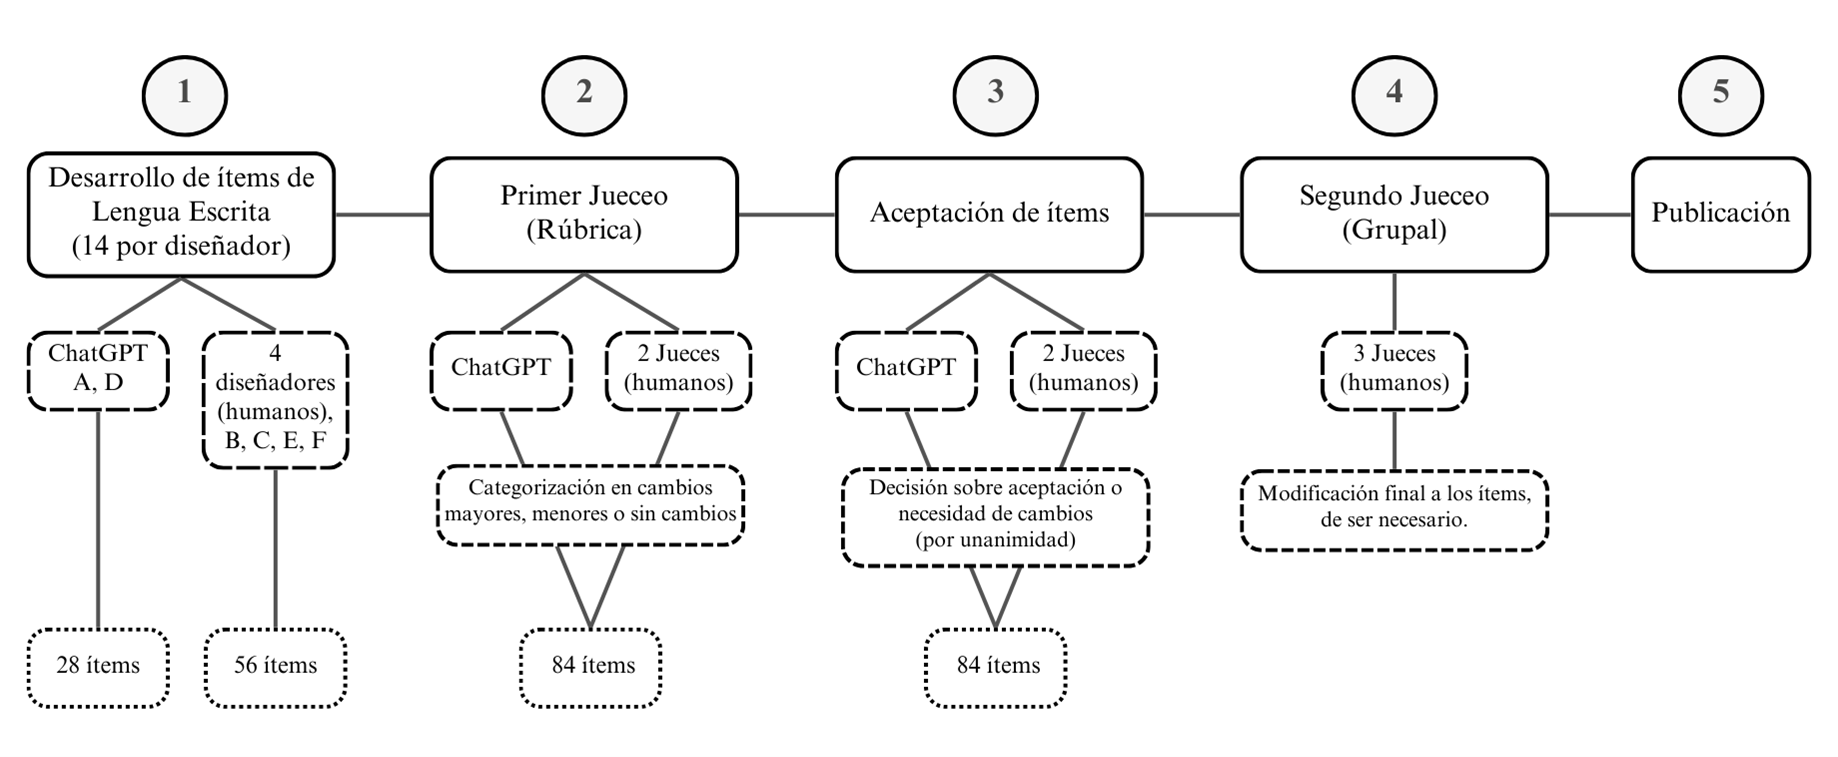
\includegraphics[width=\textwidth]{image1.png}
\caption{Proceso de evaluación y revisión de los ítems.}
\label{fig01}
\source{Elaboración propia.}
\end{minipage}
\end{figure}

Para el desarrollo de ítems se hizo uso de la IAGen ChatGPT
(\url{chat.openai.com}) en su versión de pago nombrada 4.0. Se abrieron
conversaciones por cada ítem creado, ya que todavía no estaba disponible
la posibilidad de crear un GPT con los criterios específicos para la
elaboración de ítems. En este sentido, cada ítem fue solicitado con las
características del manual de Lengua Escrita, comenzando por el uso de
la Taxonomía de \textcite{Anderson2001} para el nivel de demanda
cognitiva según la tabla de especificaciones. En cada prompt creado se
especificó:

\begin{enumerate}
	\def\labelenumi{\arabic{enumi}.}
	\item
	Identificación del contenido a evaluar
	\item
	Descripción del contenido a evaluar:
	
	\begin{enumerate}
		\def\labelenumii{\alph{enumii}.}
		\item
		Interpretación
		\item
		Ejemplos
		\item
		Delimitación del contenido
		\item
		Conocimientos y habilidades previas
		\item
		Actividades cognoscitivas
	\end{enumerate}
	\item
	Plantilla del ítem:
	
	\begin{enumerate}
		\def\labelenumii{\alph{enumii}.}
		\item
		Estructura base del ítem
		\item
		Características del texto
		\item
		Estructura y descripción de respuesta correcta y distractores.
	\end{enumerate}
	\item
	Peculiaridades de la plantilla:
	
	\begin{enumerate}
		\def\labelenumii{\alph{enumii}.}
		\item
		Base del ítem
		\item
		Vocabulario empleado
		\item
		Edición
		\item
		Peculiaridades de los distractores
	\end{enumerate}
	\item
	Bibliografía consultada y a consultar
\end{enumerate}

Por otro lado, la evaluación de los ítems fue realizada por dos jueces
humanos y por ChatGPT, siguiendo el modelo de evaluación de contenido
descrito por \textcite{Haladyna2004} y \textcite{Lynn1986}. Los jueces evaluaron cada
ítem en términos de necesidad de cambios, calidad de distractores y
aceptabilidad general del ítem. Ante esto, es importante resaltar que el
método utilizado para la evaluación de los ítems fue a doble ciego; a
ChatGPT tampoco se le indicó si quien elaboró el ítem era un ser humano
o una IAGen. Este proceso de evaluación se alinea con las
recomendaciones de \textcite{Nitko2011} sobre la importancia de una
revisión integral en la construcción de ítems de evaluación.

Los jueces evaluaron los ítems con una rúbrica (véase \Cref{tab-01}), por lo
que en esta etapa no interactuaron entre sí. Al final debían señalar si
el ítem debiese ser aceptado, aceptado con modificaciones o, bien,
podían descartarlo. Asimismo, a ChatGPT se le solicitó evaluar cada uno
de los ítems con la rúbrica disponible; es importante destacar que era
necesario tener una conversación diferente por cada ítem evaluado,
puesto que su capacidad de recordar la rúbrica era corta; es posible que
en la actualidad haya mejorado, por lo que se tiene que seguir probando
esta herramienta.



\begin{table}[!htpb]
\centering
\small
\caption{Dimensiones de la rúbrica.}
\label{tab-01}
\begin{tabular}{ll}
\toprule
Dimensiones & Elementos Clave \\
\midrule
\multirow{2}{*}{Claridad y Pertinencia del Contenido} & - Información necesaria y clara \\
    & - Tema comprensible para el público objetivo \\
\multirow{2}{*}{Neutralidad y Accesibilidad} & - Libre de sesgos\\
	& - Inclusión de imágenes/gráficas claras \\
\multirow{2}{*}{Concisión y Formato} & - Longitud adecuada del texto\\
		& - Cumplimiento de las especificaciones de formato \\
\multirow{2}{*}{Alineación Curricular} & - Congruencia con especificaciones\\
	& - Adecuación al nivel cognitivo y al público objetivo \\
\multirow{2}{*}{Claridad Disciplinar y Enfoque} & - Brevedad y claridad situacional\\
	& - Presentación directa y positiva \\
\multirow{3}{*}{Redacción y Ortografía} & - Claridad en la redacción\\
	& - Uso de vocabulario y ortografía adecuados\\
	& - Ausencia de sesgos y temas delicados \\
\multirow{3}{*}{Estructura de Respuestas} & - Uniformidad y plausibilidad de las opciones\\
	& - Ausencia de pistas indebidas\\
	& - Consistencia gramatical \\
Formato y Presentación & - Uso correcto de elementos de formato \\
\bottomrule
\end{tabular}
\source{Elaboración propia.}
\end{table}

Los resultados de las evaluaciones reflejaron una gama de decisiones,
desde la aceptación de ítems sin cambios hasta la sugerencia de
modificaciones en menor o mayor grado; o bien, el rechazo del ítem.
Estas decisiones se basaron en criterios establecidos por expertos en
evaluación educativa, como la relevancia, claridad y justicia de los
ítems \cite{Downing2003}.

Además, algunos ítems fueron seleccionados para un segundo jueceo
grupal, reflejando la metodología de revisión colaborativa sugerida por
\textcite{Stiggins2001}, lo cual permite una evaluación más profunda y detallada
en casos donde los ítems presentan desafíos particulares o requieren
ajustes más significativos. En este segundo jueceo se volvió a hacer uso
de la rúbrica, pero escuchando las observaciones de los participantes,
además se añadió a un tercer juez para tener una mejor variedad y
perspectiva sobre el jueceo.

Una vez finalizado este segundo jueceo en versión grupal, se procedió al
proceso de publicación de los ítems en su versión impresa para su
aplicación en el mes de noviembre del año 2023, como parte del proceso
de selección de ingreso a la universidad. En esta aplicación se contó
con la participación de 2,263 sustentantes, siendo 50.06~\% mujeres y
49.93~\% hombres. Los resultados de aplicación del modelo Rasch, el cual
es idóneo para medir actitudes, habilidades o personalidad
(Tristán-López, 1998), se presentan en el Anexo 1, donde todos los ítems
resultaron con índices favorables conforme a los principios de la Teoría
de Respuesta al Ítem (TRI).

Por otro lado, para el análisis del comportamiento de los jueces se
realizaron los siguientes pasos:

\begin{enumerate}[label=\Alph*)]
\item Para observar las diferencias entre el jueceo a ítems diseñados por humanos y ChatGPT
\begin{enumerate}[label=\arabic*.]
\item Preparación de datos, de forma categórica.
\item Prueba Chi-cuadrado en SPSS, siguiendo las recomendaciones de \cite{Field2013}.
\item Preparación de datos, de forma numérica para proceder a un ANOVA o
bien la prueba de Kruskal-Wallis \cite{Field2013,Howell2012}.
\item Prueba de normalidad en SPSS; el resultado fue no normal, por lo que
se procedió a la prueba de Kruskal-Wallis con las variables: Creadores
(Humano, ChatGPT), Juez A, Juez B, ChatGPT; además se aplicó la prueba
U de Mann-Whitney (Field, 2013) realizando la prueba por cada una de
las variables para revisar si había alguna variación. Todos ellos con
el \emph{software} SPSS.
\item Análisis de resultados con estadísticos básicos comparativos.
\end{enumerate}

\item Para observar la concordancia entre jueces
\begin{enumerate}[label=\arabic*.]
\item Prueba de Kappa de Cohen \cite{McHugh2012}, entre jueces: A y B, A y
ChatGPT, B y ChatGPT, a través del \emph{software} SPSS.
\item Prueba alfa de Krippendorff \cite{Hayes2007}: A, B y ChatGPT, a través del software R (Versión 2023.12.0+369), con	paquetería tidyverse e IRR.
\item Análisis de resultados con estadísticos básicos comparativos.
\end{enumerate}

\end{enumerate}
\section{Análisis y resultados}\label{sec-análisisyresultados}

Los resultados de este estudio se representan organizados según los
criterios de análisis establecidos. En primer lugar, se muestran los
números de artículos publicados por periodos temporales, es decir, por
años naturales. En ellos se evidencia un aumento progresivo anual de la
producción, y 2021 como el año con el incremento más pronunciado \Cref{tab-01}.

\begin{table}[htbp]
\centering
\begin{threeparttable}
\caption{Número de artículos por año.}
\label{tab-01}
\begin{tabular}{lll}
\toprule
Año & Artículos & Diferencia\\
\midrule
2019 & 26 & - \\
2020 & 28 & 2 \\
2021 & 40 & 12\\
2022 & 51 & 11\\
\bottomrule
\end{tabular}
\source{Elaboración propia.}
\end{threeparttable}
\end{table}

A partir de 2021 se observa una mayor preocupación por explorar nuevas
fórmulas narrativas. Encontramos una razón para ello en la crisis del
COVID-19. De acuerdo con diversos autores \cite{monroy_retos_2021,torras_virgili_emergency_2021,una_martin_aproximacion_2020,vilhelm_rios_didactica_2022}, consideramos que la
pandemia y la crisis sanitaria reformularon muchos planteamientos
pedagógicos tradicionales, generando la necesidad de experimentar con
modelos más flexibles, personalizados, con tecnologías y metodologías
más innovadoras.

El número de citas de los artículos es muy variable, y no puede
establecerse un patrón de comportamiento, ni correlación entre las
fechas de publicación y el impacto de los artículos. Aunque generalmente
los artículos más antiguos suelen tener mayor número de citas, en el
caso que nos ocupa los dos artículos más destacados fueron publicados en
2021. Entre toda la producción seleccionada, podemos destacar un trabajo
que alcanza más de sesenta citas, y otros siete con cifras superiores o
iguales a veinte \Cref{tab-02}

\begin{table}[htbp]
\centering
\begin{threeparttable}
\caption{Número de citas por año.}
\label{tab-02}
\begin{tabular}{lllll}
\toprule
\multicolumn{1}{c}{Artículo} & \multicolumn{4}{c}{Citas por año} \\
  &2019& 2020& 2021& 2022\\
\midrule
Secundo, Mele, Vecchio, Elia, Margherita, \& Ndou (2021) &-& - &16& 51\\
Agbo, Oyelere, Suhonen, \& Tukianen (2021)& -& - &12 &25\\
Kerr, \& Lawson (2020)& - &6& 16 &11\\
Flórez-Aristizábal \& Fardoun (2019)& 3& 4 &7& 12\\
Naul, \& Liu (2020) &- &1& 9& 15\\
Sarnok, Wannapiroon, \& Nilsook (2019) &1 &4& 8& 10\\
Kaeophanuek, Na-Songkhla, \& Nilsook (2019) & 2 & 4& 8& 7\\
\bottomrule
\end{tabular}
\source{Elaboración propia.}
\end{threeparttable}
\end{table}

Atendiendo al número de citas, debemos destacar tres artículos que están
liderando la tendencia en investigación sobre el \emph{storytelling}
mediado por el uso de tecnología y sus posibilidades pedagógicas. Se
trata de los trabajos de \cite{secundo_threat_2021,agbo_scientific_2021,kerr_augmented_2020}.

El primero de ellos surge en el contexto de crisis del COVID-19, y en él
se abordan los principales retos tecnológicos que la pandemia generó en
el ámbito educativo. Los autores ilustran el rediseño de un programa de
aprendizaje para emprendedores, aprovechando las tecnologías digitales y
a nivel práctico, aportan ideas para remodelar los programas
universitarios tradicionales, preparándolos para abordar emergencias
futuras.

El segundo artículo ofrece una amplia revisión bibliográfica en la que
se examina el panorama de la investigación sobre los Entornos
Inteligentes de Aprendizaje, mediante un análisis bibliométrico. El
resultado de este análisis indica que el primer artículo sobre esta
nueva realidad se publicó en 2002, lo que supuso el inicio en la
exploración de este campo. Los Entornos Inteligentes de Aprendizaje
aluden a entornos físicos enriquecidos con dispositivos digitales,
sensibles al contexto y adaptativos, para promover un aprendizaje más
rápido y eficaz \cite{koper_conditions_2014}. Su análisis temático muestra que la narración digital y sus componentes asociados, como la realidad virtual, el pensamiento crítico y los Juegos Serios, que son juegos creados para proporcionar un contexto de entretenimiento y auto-fortalecimiento con
el que motivar, educar y entrenar a los jugadores  \cite{chipia_lobo_juegos_2011}. Consideramos que se trata de dos líneas de investigación emergentes.

Por último, en el artículo de \cite{kerr_augmented_2020}, se describe el
desarrollo de un prototipo de Realidad Aumentada, creado para formar a
estudiantes en los principios básicos de la arquitectura paisajística.
El enfoque principal de los autores se centra en proponer nuevas
prácticas de narración digital a través de experiencias situadas. De
este trabajo inferimos la necesidad de mejorar los programas de
formación docente para capacitar a los futuros maestros en la
integración de las tecnologías inmersivas, como también indica \cite{figueroa_fusionando_2021}.

El tercer indicador hace referencia a las autorías, y nos permite
destacar a los investigadores que más han aportado en el campo objeto de
estudio. En la siguiente tabla mostramos sus nombres y filiación
institucional, a través de la cual podemos observar una gran
representación de Australia y Malasia país que, junto a Tailandia,
lidera sus investigaciones desde universidades centradas en el
desarrollo tecnológico \Cref{tab-03}.

Este dato se corrobora al confrontarlo con las instituciones destacadas
en la investigación sobre \emph{Storytelling} \Cref{tab-04}.

\begin{table}[htbp]
\centering
\begin{threeparttable}
\caption{Investigadores destacados.}\label{tab-03}
\begin{tabular}{lll}
\toprule
Investigador & Filiación & Artículos\\
\midrule
Nilsook, Prachyanun &King Mongkut´s University of Technology & 3\\
Buendgens-Kosten, Judith & Goethe-Universität Frankfurt am Main & 2\\
Chubko, Nadezhda & Edith Cowan University & 2\\
Cornillie, Frederik & KU Leuven & 2 \\
Girmen, Pınar &  Eskişehir Osmangazi Üniversitesi & 2\\
Kantathanawat, Thiyaporn K. & Mongkut's Institute of Technology Ladkrabang & 2\\
Kantathanawat, Thiyaporn K. & Mongkut\textquotesingle s Institute of Technology Ladkrabang & 2\\
Lummis, Geoff W. & Edith Cowan University& 2\\
Macleroy, Vicky & Goldsmiths, University of London &2\\
McKinnon, David H. & Edith Cowan University & 2\\
Morris, Julia Elizabeth & Edith Cowan University & 2\\
\bottomrule
\end{tabular}
\source{Elaboración propia.}
\end{threeparttable}
\end{table}


Al analizar las filiaciones (\Cref{tab-04}) de los principales autores y producción por
países, encontramos en Europa y América del Norte el mayor volumen de
aportaciones. El continente americano, lidera las investigaciones que
relacionan el \emph{Storytelling} con el ámbito de la medicina y la
salud, aunque también hay una gran representación europea debido a las
aportaciones de Reino Unido. En lo referente al campo de las ciencias
sociales, Europa es quien lidera y marca las tendencias. España, que
ocupa el cuarto puesto de la tabla en número de aportaciones por países
con un total de catorce artículos, destaca por su contribución a los
campos relacionados con la aplicación de la narrativa en entornos
digitales, nuevos soportes, y en el uso de metodologías activas. En este
sentido, podríamos señalar a este país como uno de los líderes en la
investigación sobre innovación y tecnología educativa. Este interés por
el \emph{Storytelling} aplicado a metodologías activas y recursos
digitales, continúa aumentando y ha sido identificado en otros estudios
recientes vinculados a universidades españolas \cite{sanchez-rivas_narrative-based_2022,sanchez_rivas_experiencia_2023}.

\begin{table}[htbp]
\centering
\begin{threeparttable}
\caption{Instituciones destacadas.}
\label{tab-04}
\begin{tabular}{lll}
\toprule
Institución & País & Artículos \\
\midrule
Universiti Kebangsaan & Malasia & 3\\
Goldsmiths, University of London & Reino Unido & 3\\
Universiti Teknologi Malaysia & Malasia & 3\\
King Mongkut\textquotesingle s Institute of Technology Ladkrabang &
Tailandia &3\\
Edge Hill University & Reino Unido & 3\\
National and Kapodistrian University of Athens & Grecia & 3\\
King Mongkut\textquotesingle s University of Technology North Bangkok&
Tailandia &3\\
Universitat Oberta de Catalunya & España & 2\\
Universiti Utara Malaysia & Malasia & 2\\
David Geffen School of Medicine at UCLA & Estados Unidos & 2\\
Universidad de Oviedo& España & 2\\
\bottomrule
\end{tabular}
\source{Elaboración propia.}
\end{threeparttable}
\end{table}

 En lo que respecta a la producción por países, Estados Unidos ocupa la primera posición con veintiuna aportaciones, seguido de Reino Unido y Australia. España ocupa la cuarta posición de la tabla con una aportación de catorce artículos, el mismo número que Australia \Cref{tab-05}.
 
\begin{table}[htbp]
\centering
\begin{threeparttable}
\caption{Producción por países.}
\label{tab-05}
\begin{tabular}{ll}
\toprule
País & Artículos \\
\midrule
Estados Unidos & 21\\
Reino Unido & 19\\
Australia & 14\\
España & 14\\
Grecia & 11\\
Malasia & 10\\
Canadá & 9 \\
Italia & 9\\ 
\bottomrule
\end{tabular}
\source{Elaboración propia.}
\end{threeparttable}
\end{table}

Si atendemos a las líneas de investigación abiertas en relación con el
\emph{Storytelling,} advertimos que su estudio se aborda desde
diferentes disciplinas. Aunque el enfoque de las investigaciones siempre
tiene una perspectiva pedagógica, podemos asegurar que el tratamiento
científico de las mismas se acomete desde una perspectiva
multidisciplinar \Cref{tab-06}.

\begin{table}[htbp]
\centering
\begin{threeparttable}
\caption{Producciones por disciplina científica.}
\label{tab-06}
\begin{tabular}{ll}
\toprule
País & Artículos \\
\midrule
Ciencias Sociales & 107\\
Ciencias Informáticas & 40\\
Artes y Humanidades & 22\\
Ingeniería & 16\\
Medicina & 15\\
Psicología & 15\\
Administración y negocios & 6\\
Ciencias Medioambientales & \\
Ciencia de Materiales & 5\\
Ciencias de la Salud &5\\
\bottomrule
\end{tabular}
\source{Elaboración propia.}
\end{threeparttable}
\end{table}

A la hora de abordar nuestro análisis cualitativo, y dar respuesta a
nuestra primera pregunta de investigación, se realizó un análisis de los
campos de estudio y de los contenidos desde los que se abordaban los
diferentes artículos publicados, es decir, aquellos ámbitos con mayor
interés en el uso de historias como recurso didáctico. Las Ciencias
Sociales, las Ciencias Informáticas y las Artes y Humanidades fueron las
áreas más productivas. Cabe destacar que, si a la medicina le sumamos
las publicaciones de otros campos afines como el de las ciencias de la
salud o el de la psicología, ocuparían el tercer puesto. Esto es debido
a la gran cantidad de estudio de casos que utilizan estas ciencias tanto
para enseñar, como para contrastar información en el desempeño de su
trabajo.

A esta revisión de naturaleza cuantitativa, se añadió otra de tipo
documental, para responder a nuestra segunda pregunta e identificar las
finalidades pedagógicas de las líneas temáticas más investigadas en cada
una de las principales áreas de estudio. Los trabajos analizados podrían
organizarse en tres grandes bloques (\Cref{tab-07}). En primer lugar, aquellos que ponen su foco en el proceso de aprendizaje y utilizan las técnicas vinculadas a las historias para mejorar el proceso didáctico. Dentro de esta vertiente, encontramos una gran tendencia a trasladar los modelos
clásicos de la narración a nuevos medios, soportes y tecnologías. En
segundo lugar, contamos con una gran producción de trabajos enfocados en
la transmisión de valores, concienciación con el medio ambiente, con la
inclusión y la necesidad de eliminar fronteras tecnológicas, sociales, y
étnicas. Por último, encontramos una línea dedicada a utilizar la
narración como cauce terapéutico, destinando sus estrategias y recursos
a mejorar la salud física y mental de las personas.

\begin{table}[htbp]
\centering
\begin{threeparttable}
\caption{Principales finalidades pedagógicas de la narración de historias en los artículos analizados.}
\label{tab-07}
\begin{tabular}{ll}
\toprule
Bloque 1 & Narración de historias como parte del proceso de enseñanza y
aprendizaje.\\
Bloque 2 & Narración de historias como medio de transmisión de valores.\\
Bloque 3 & Narración de historias como cauce terapéutico.\\
\bottomrule
\end{tabular}
\source{Elaboración propia.}
\end{threeparttable}
\end{table}

Al enfrentarnos a nuestra tercera pregunta de investigación, y analizar
los conceptos más mencionados en cada uno de los bloques anteriormente
descritos, en el primero de ellos descubrimos un creciente interés en la
comunidad científica por la necesidad de construir historias que
contribuyan al éxito en la aplicación de las denominadas metodologías
activas en el aula. De esta manera, los términos Aprendizaje Basado en
Proyectos, el Aprendizaje Basado en Resolución de Problemas y el
Aprendizaje Cooperativo, son habituales en los trabajos analizados. Del
mismo modo, se identifica un gran volumen de referencias sobre el uso de
la tecnología y los recursos digitales como herramientas de trabajo. En
este sentido, los términos \enquote{Robot}, \enquote{Narrativa Digital}, \enquote{Mapa Digital}, \enquote{Social Media}, \enquote{Dispositivos móviles}, o \enquote{Realidad Aumentada} son los más mencionados.

Con respecto a los trabajos centrados en la concienciación y transmisión
de valores, el concepto de \enquote{Desarrollo Sostenible} es el más repetido,
y también identificamos un gran interés en lo referido a crear
estrategias dirigidas a frenar el cambio climático, la inclusión de
minorías y la conservación del patrimonio inmaterial de las diferentes
culturas. También detectamos una notable producción enfocada en el
intento de disminuir la brecha digital y la igualdad de oportunidades.

En cuanto al tercer bloque, al analizar el área de la salud y el ámbito
terapéutico, los principales ejes de interés se posicionaron entorno a
conceptos como el acompañamiento a pacientes, el estudio de casos de
éxito en medicina, la atención a niños con trastornos del espectro
autista, las terapias psicológicas con animales y el arte, y el refuerzo
de la autoestima.

Además, cabe destacar que desde todas las áreas específicas de
conocimiento se hallaron dos grandes tendencias. La primera de ellas
referida al concepto \enquote{Narración Transmedia}, entendida como un
proceso en el que los elementos integrales de una historia se dispersan
sistemáticamente a través de múltiples canales de distribución con el
fin de crear una experiencia de entretenimiento unificada y coordinada
\cite{jenkins_transmedia_2010}. El otro núcleo de interés está relacionado con la pandemia del COVID-19, y numerosos artículos inciden en la necesidad de
estructurar la narración para mantener la atención de los estudiantes
durante el proceso de \enquote{e-Learning} o \enquote{Aprendizaje a distancia}, así como de la importancia de emplear la tecnología para conseguirlo. Por último, cabe destacar otros dos campos que están presentes en un gran número de estudios y generando tendencia, que son los \enquote{Entornos Inteligentes de Aprendizaje} y la \enquote{Realidad Aumentada}.

Desde el punto de vista metodológico, encontramos una mayoría de
estudios mixtos, que combinan técnicas cuantitativas y cualitativas,
entre las que destacan los estudios etnográficos. Con respecto a las
investigaciones que derivan de las ramas del área de la salud,
identificamos una gran producción en forma de estudios de casos.

\section{Discusión y conclusiones}\label{sec-discusiónyconclusiones}

Partiendo de los resultados obtenidos, consideramos que se refuerza un
planteamiento, ya apuntado por otros autores \cite{alfian_role_2021,sidorenko-bautista_use_2020}, que
sostiene que las narrativas deben cambiar para adaptarse a los nuevos
medios, y que los medios están cambiando continuamente para adaptarse a
las narrativas. En este sentido, se observa un gran interés de la
comunidad científica por adaptar las técnicas clásicas de la narración a
los nuevos medios, soportes, tecnologías y entornos, para logar conectar
con sus audiencias. La necesidad de vehicular contenidos a través de
estructuras narrativas creíbles resulta esencial ya que, de acuerdo con
\cite{vergara2020herramientas}, podemos decir que si algo nos
caracteriza desde el punto de vista cultural es que somos depredadores
de buenas historias.

Como podemos observar, el interés por el \emph{Storytelling} ha superado
la barrera de las Ciencias Sociales, posicionándose como método de
transmisión de conocimiento en diversas disciplinas. El
\emph{Storytelling} es una herramienta poderosa que ha sido utilizada
durante siglos en una variedad de ámbitos, desde la literatura hasta la
publicidad, desde la política hasta la psicología. Su capacidad para
inspirar, educar y entretener va mucho más allá de las ciencias sociales
\cite{haven_story_2007}.

Los hallazgos que hemos realizado nos permiten concluir que la narrativa
sigue siendo fundamental para la articulación de contenidos y el proceso
de enseñanza y aprendizaje. La comunidad científica muestra un gran
interés por adaptar la narrativas y técnicas del \emph{Storytelling} a
los nuevos escenarios educativos, metodologías y herramientas
tecnológicas. La continua exploración de las posibilidades de estas
técnicas está despertando el interés de diferentes disciplinas que
persiguen beneficiarse del carácter pedagógico de las historias.

Podemos establecer otra línea de conclusiones en relación con las
temáticas que se abordan en las historias. Hemos detectado un gran
interés de la comunidad científica por construir narrativas eficaces que
puedan ayudar a comprender las claves del cambio climático. En este
sentido, resulta interesante la vía abierta por diversos trabajos \cite{arnoud_climate_2018,bloomfield_climate_2021,de_meyer_transforming_2021,moezzi_using_2017} que recomiendan trasladar, utilizando
técnicas de comunicación efectiva, estas narrativas climáticas a todas
las esferas de la sociedad, y no solo al ámbito educativo.

Desde la perspectiva didáctica, se hace evidente el interés por crear
propuestas metodológicas específicas que permitan aprovechar todo el
potencial del \emph{Storytelling} en el aula. Los métodos activos son,
en todos los casos, las opciones preferidas. Entendemos que se trata de
una relación lógica, ya que el Storytelling guarda una relación de
coherencia con los rasgos propios del aprendizaje activo (implicación
emocional, cooperación, creatividad, búsqueda del conocimiento, etc.).
Hemos encontrado diferentes estrategias metodológicas para utilizar las
historias como recurso didáctico. Muchas se integran en el método
didáctico Aprendizaje Basado en Historias.

Otros de los fenómenos a los que la comunidad científica debe prestar
atención en el futuro es al de los \emph{Entornos Inteligentes de
Aprendizaje} y a \emph{la Narración transmedia}. De todas estas nuevas
vías, surgen fortalezas como el potencial pedagógico de las narrativas
aplicadas al pensamiento reflexivo o a los nuevos medios digitales \cite{kim_digital_2021,yasar__2022} y otros debates éticos, como la
moralidad de utilizar técnicas de manipulación, como podría considerarse
el \emph{Storytelling} dentro del contexto de las redes sociales tras
demostrarse los efectos negativos que estas producen en la salud mental
\cite{sheldon_dark_2019}.

En cuanto al uso de la tecnología que todas estas metodologías
combinadas con narrativas propician, se imponen con claridad
instrumentos como los dispositivos móviles y la realidad aumentada. En
este sentido, numerosos autores \cite{aurelia_survey_nodate,dunleavy_augmented_2014,nam_designing_2015,nobrega_mobile_2017} apuntan al potencial de la combinación de ambas tecnologías como un buen modelo de enseñanza debido a que cualquier lugar u objeto del mundo real puede integrarse en una historia, estimulando la imaginación del participante. Aunque también señalan que existen algunas barreras que impiden a los usuarios participar activamente en este tipo de actividades, como la
necesidad de disminuir la brecha digital y el elevado coste de los
dispositivos y la tecnología.

Al contrastar nuestra revisión con otras similares, podemos comprobar
que las conclusiones confluyen en varios aspectos. El primero de ellos
sería en la positiva percepción sobre la aplicación de la narración
digital de historias por parte de los estudiantes. Esta idea ha sido
destacada en otras revisiones que también señalan el efecto novedad como
posible artífice de esta aceptación. Se propone continuar investigando
para ver cómo se desarrolla esta relación en el futuro. El segundo
aspecto a tener en cuenta sería la necesidad de formar a los docentes en
el uso de los entornos digitales y la creación, ya que la narración de
historias continúa capturando la atención de audiencias, convirtiéndose
en un aliado indispensable de cualquier proceso didáctico y formativo,
por lo que necesitamos formar a nuestros docentes \cite{chikasanda_enhancing_2013,lawless_professional_2007}.

En relación con futuras líneas de investigación, cabe apuntar que el
importante índice de experimentación didáctica que hemos encontrado,
unido a la necesidad de una constante adaptación de las narrativas a los
nuevos entornos inteligentes y digitalizados, derivarán en nuevas formas
de enseñar y aprender en el futuro, a las que la comunidad científica
deberá prestar atención para evaluar su potencial y medir su eficacia.


\printbibliography\label{sec-bib}
%conceptualization,datacuration,formalanalysis,funding,investigation,methodology,projadm,resources,software,supervision,validation,visualization,writing,review
\begin{contributors}[sec-contributors]
\authorcontribution{Enrique Sánchez Rivas}[conceptualization,methodology,resources,writing]
\authorcontribution{Manuel Fernando Ramos Núnez}[conceptualization,datacuration,investigation,validation,writing]
\authorcontribution{José Sánchez Rodríguez}[formalanalysis,review,supervision]
\authorcontribution{María Rubio-Gragera}[formalanalysis,review,supervision]
\end{contributors}
\end{document}
